% This is a Basic Assignment Paper but with like Code and stuff allowed in it, there is also url, hyperlinks from contents included. 

\documentclass[11pt]{article}

% Preamble

\usepackage[margin=1in]{geometry}
\usepackage{amsfonts, amsmath, amssymb}
\usepackage{fancyhdr, float, graphicx}
\usepackage[utf8]{inputenc} % Required for inputting international characters
\usepackage[T1]{fontenc} % Output font encoding for international characters
\usepackage{fouriernc} % Use the New Century Schoolbook font
\usepackage[nottoc, notlot, notlof]{tocbibind}
\usepackage{listings}
\usepackage{xcolor}
\usepackage{blindtext}
\usepackage{hyperref}
\hypersetup{
    colorlinks=true,
    linkcolor=black,
    filecolor=magenta,      
    urlcolor=cyan,
    pdfpagemode=FullScreen,
    }

\definecolor{codegreen}{rgb}{0,0.6,0}
\definecolor{codegray}{rgb}{0.5,0.5,0.5}
\definecolor{codepurple}{rgb}{0.58,0,0.82}
\definecolor{backcolour}{rgb}{0.95,0.95,0.92}

\lstdefinestyle{mystyle}{
    backgroundcolor=\color{backcolour},   
    commentstyle=\color{codegreen},
    keywordstyle=\color{magenta},
    numberstyle=\tiny\color{codegray},
    stringstyle=\color{codepurple},
    basicstyle=\ttfamily\footnotesize,
    breakatwhitespace=false,         
    breaklines=true,                 
    captionpos=b,                    
    keepspaces=true,                 
    numbers=left,                    
    numbersep=5pt,                  
    showspaces=false,                
    showstringspaces=false,
    showtabs=false,                  
    tabsize=2
}

\lstset{style=mystyle}

% Header and Footer
\pagestyle{fancy}
\fancyhead{}
\fancyfoot{}
\fancyhead[L]{\textit{\Large{Information and Cycbersecurity - 2nd Year B. Tech}}}
%\fancyhead[R]{\textit{something}}
\fancyfoot[C]{\thepage}
\renewcommand{\footrulewidth}{1pt}



% Other Doc Editing
% \parindent 0ex
%\renewcommand{\baselinestretch}{1.5}

\begin{document}

\begin{titlepage}
    \centering

    %---------------------------NAMES-------------------------------

    \huge\textsc{
        MIT World Peace University
    }\\

    \vspace{0.75\baselineskip} % space after Uni Name

    \LARGE{
        Information and Cybersecurity\\
        Second Year B. Tech, Semester 1
    }

    \vfill % space after Sub Name

    %--------------------------TITLE-------------------------------

    \rule{\textwidth}{1.6pt}\vspace*{-\baselineskip}\vspace*{2pt}
    \rule{\textwidth}{0.6pt}
    \vspace{0.75\baselineskip} % Whitespace above the title



    \huge{\textsc{
            Email Security using - PGP
        }} \\



    \vspace{0.5\baselineskip} % Whitespace below the title
    \rule{\textwidth}{0.6pt}\vspace*{-\baselineskip}\vspace*{2.8pt}
    \rule{\textwidth}{1.6pt}

    \vspace{1\baselineskip} % Whitespace after the title block

    %--------------------------SUBTITLE --------------------------	

    \LARGE\textsc{
        Lab Assignment 8
    } % Subtitle or further description
    \vfill

    %--------------------------AUTHOR-------------------------------

    Prepared By
    \vspace{0.5\baselineskip} % Whitespace before the editors

    \Large{
        Krishnaraj Thadesar \\
        Cyber Security and Forensics\\
        Batch A1, PA 20
    }


    \vspace{0.5\baselineskip} % Whitespace below the editor list
    \today

\end{titlepage}


\tableofcontents
\thispagestyle{empty}
\clearpage

\setcounter{page}{1}

\section{Aim}
Demonstrate Email Security using - PGP or S/MIME for Confidentiality, Authenticity and Integrity.

\section{Objectives}
To learn authentication technique for access control

\section{Theory}

\subsection{PGP}

\begin{enumerate}
    \item PGP (Pretty Good Privacy) is a data encryption and decryption computer program that provides cryptographic privacy and authentication for data communication. PGP is used for signing, encrypting, and decrypting texts, e-mails, files, directories, and whole disk partitions and to increase the security of e-mail communications.
    \item Phil Zimmermann developed PGP in 1991. PGP and similar software follow the OpenPGP standard (RFC 4880) for encrypting and decrypting data.
    \item PGP encryption uses a serial combination of hashing, data compression, symmetric-key cryptography, and, finally, public-key cryptography; each step uses one of several supported algorithms. Each public key is bound to a user name and/or an e-mail address. The first version of this system was generally known as a web of trust to contrast with the X.509 system, which uses a hierarchical approach based on certificate authority and which was added to PGP implementations later. Current versions of PGP encryption include both options through an automated key management server.
    \item PGP encryption should only be used with data that is transferred via file transfer applications that use secure connections. PGP should not be used with email applications that send and receive data in plain text. PGP encryption is not compatible wi    
\end{enumerate}

\subsection{Steps to Send an EMail using PGP}
\subsubsection{Generate a key Pair}

The first step is to generate a key pair consisting of a private key and a public key. The private key is kept secret and is used for decrypting messages that are encrypted using the corresponding public key. The public key is shared with others so they can encrypt messages that only the owner of the private key can decrypt.

\subsubsection{Share public keys}

In order to exchange encrypted messages, each person needs to share their public key with the other person. This can be done by sharing the key through a key server, sending the key as an email attachment, or sharing it in person.
\subsubsection{Encrypt the message}

Once the public keys have been exchanged, the sender can encrypt the message using the recipient's public key. The encrypted message can only be decrypted by the recipient using their private key.
\subsubsection{Sign the message}

The sender can optionally sign the message using their private key. This adds a digital signature to the message, which provides a way for the recipient to verify that the message was actually sent by the claimed sender, and that it has not been altered in transit.
\subsubsection{Send the message}

The encrypted and optionally signed message can now be sent to the recipient through email or another messaging service.
\subsubsection{Decrypt the message}

Upon receiving the message, the recipient can decrypt it using their private key. If the message was also signed, the recipient can verify the digital signature using the sender's public key.

These steps are shown below in Input and outputs.

\section{Platform}
\textbf{\textbf{Operating System}}: Arch Linux x86-64 \\
\textbf{\textbf{IDEs or Text Editors Used}}: Visual Studio Code\\

\section{Input and Output}

\subsection{Generated Keys}

\lstinputlisting[language=bash, caption="Krish Private Key"]{../Programs/Assignment_8/krish_private_key.txt}

\lstinputlisting[language=bash, caption="Krish Public Key"]{../Programs/Assignment_8/krish_public_key.txt}

\begin{figure}[H]
    \centering
    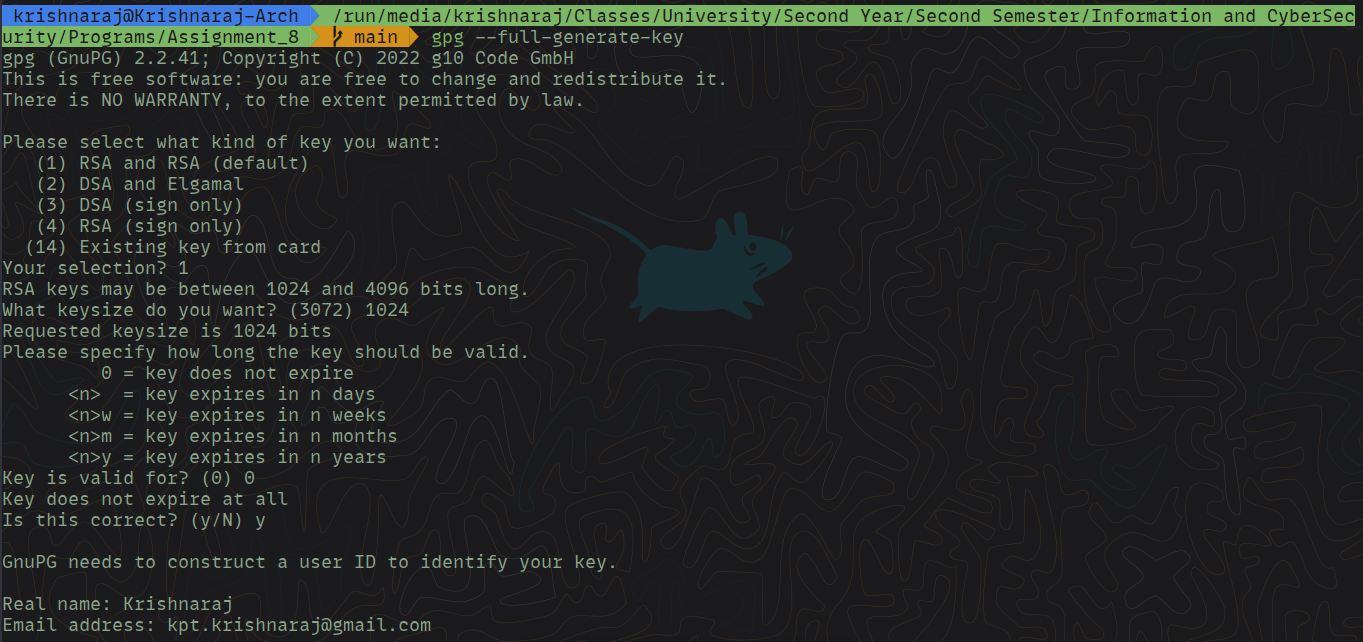
\includegraphics[width=1\textwidth]{../Programs/Assignment_8/Screenshot_on_2023-04-13_at_12-28-59.png}
    \caption{Generating Key Pairs}
\end{figure}
\begin{figure}[H]
    \centering
    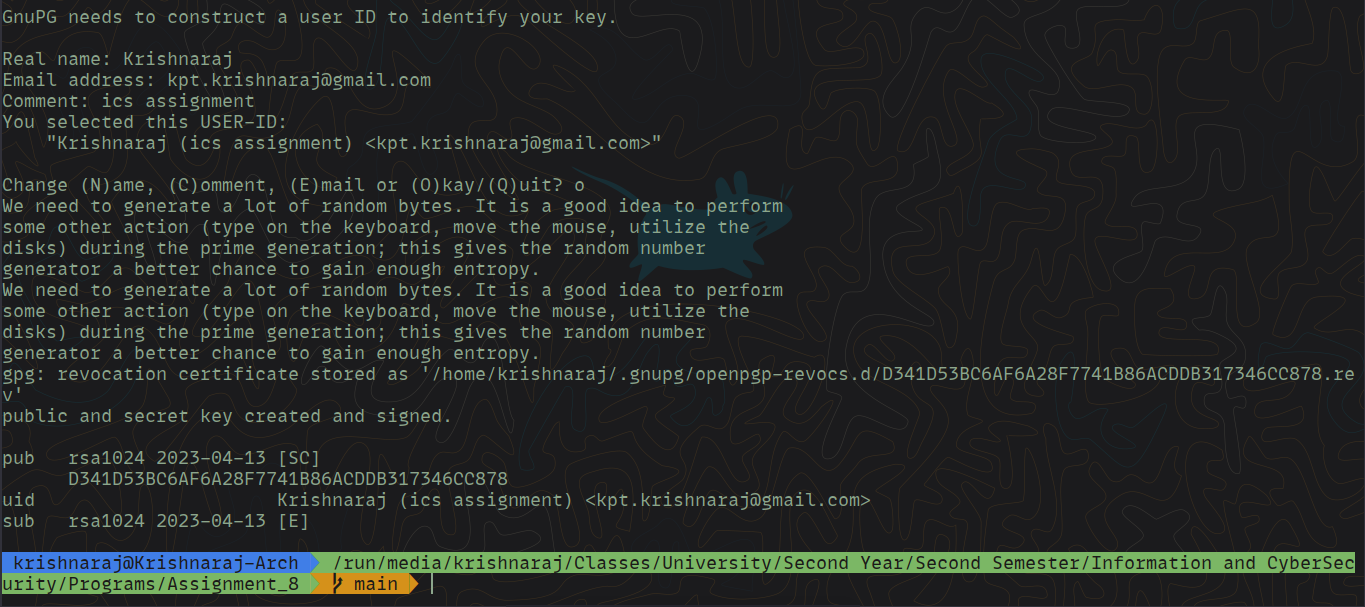
\includegraphics[width=.99\textwidth]{../Programs/Assignment_8/Screenshot_on_2023-04-13_at_12-29-06.png}
    \caption{Generating Key Pairs continued}
\end{figure}
\begin{figure}[H]
    \centering
    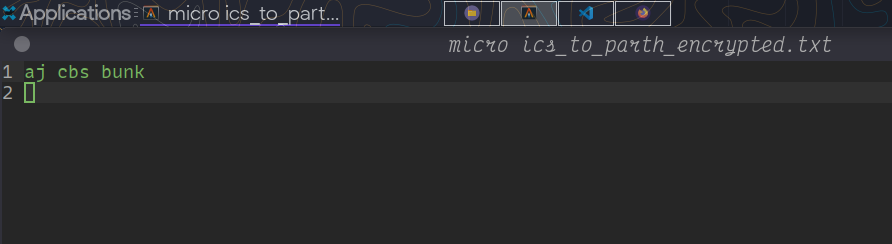
\includegraphics[width=.99\textwidth]{../Programs/Assignment_8/Screenshot_on_2023-04-13_at_12-29-34.png}
    \caption{Secret Message to Parth - Recipient - "Aj CBS Bunk"}
\end{figure}
\begin{figure}[H]
    \centering
    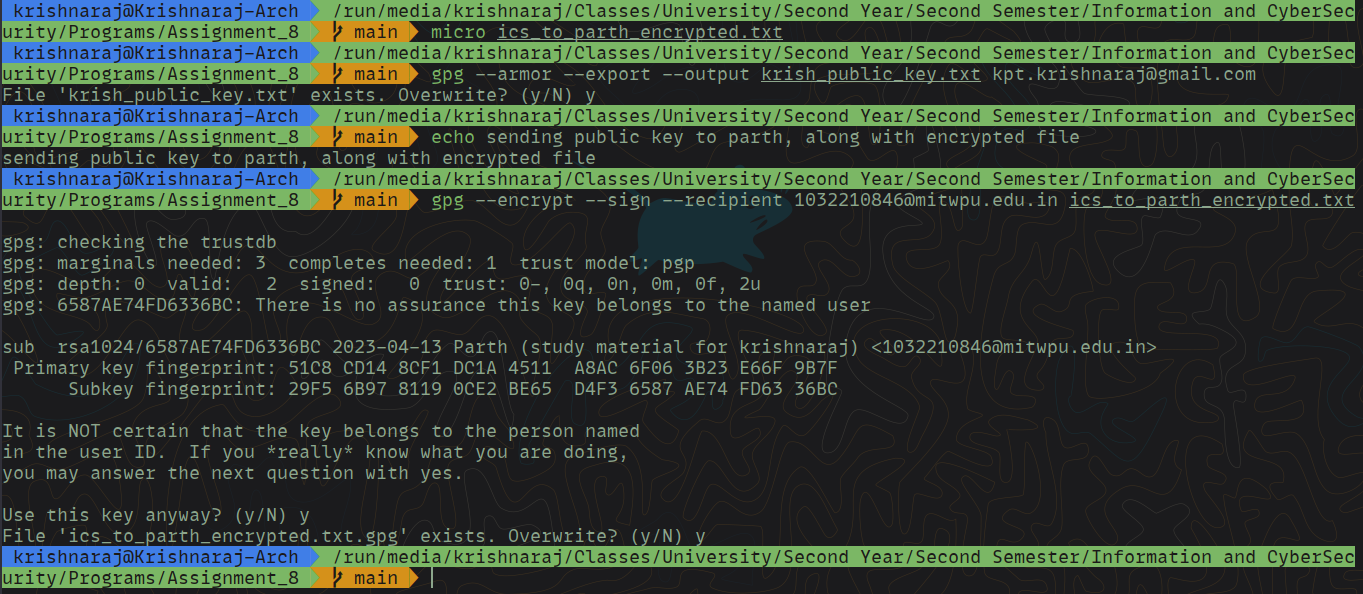
\includegraphics[width=.99\textwidth]{../Programs/Assignment_8/Screenshot_on_2023-04-13_at_12-31-43.png}
    \caption{Signing Message to Send Parth using Parth's Public Key}
\end{figure}
\begin{figure}[H]
    \centering
    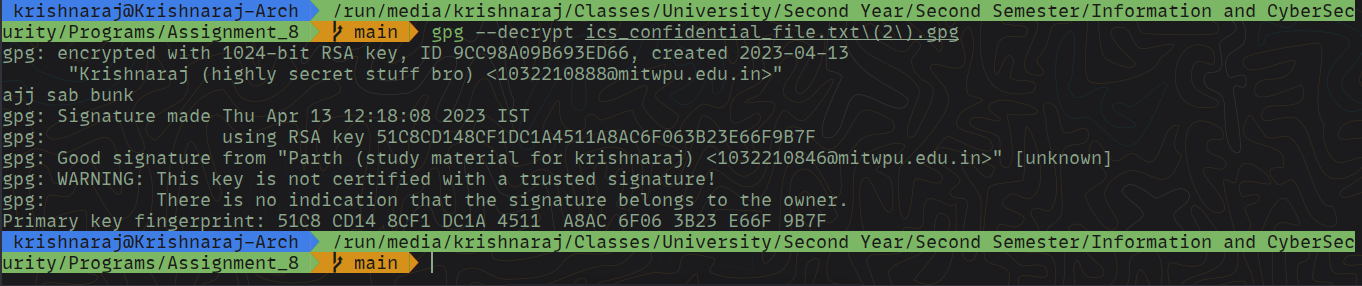
\includegraphics[width=.99\textwidth]{../Programs/Assignment_8/Screenshot_on_2023-04-13_at_12-32-03.png}
    \caption{Decrypting Message from Parth using his Public key - "Ajj Sab Bunk"}
\end{figure}

\begin{verbatim}

\end{verbatim}


% \section{Code}
% \lstinputlisting[language=Python, caption="DSA Signature Validity using PyCrypto Library"]{../Programs/Assignment_7/dsa using lib.py}

\section{Conclusion}
Thus, we have successfully implemented Email Security using - PGP or S/MIME for Confidentiality, Authenticity and Integrity.
\clearpage

\section{FAQ}

\begin{enumerate}
    \item \textbf{How email security is provided through PGP?}\\

          \begin{enumerate}
              \item PGP (Pretty Good Privacy) provides email security through a combination of encryption, digital signatures, and compression. When a user sends an email using PGP, the message is encrypted using a symmetric key algorithm.

              \item The symmetric key is then encrypted using the recipient's public key, which is obtained from a key server or a public key directory. The encrypted message and the encrypted symmetric key are then sent to the recipient, who can decrypt the message using their private key.

              \item PGP also allows users to sign their emails digitally using their private key. The digital signature provides a way for the recipient to verify that the email was actually sent by the claimed sender, and that it has not been altered in transit.
              \item In addition, PGP can compress the message before encryption, which can reduce the size of the message and make it easier to send over a slow or unreliable connection.
          \end{enumerate}

    \item \textbf{What type of encryption is PGP?}\\

          PGP uses a combination of symmetric and asymmetric encryption. The symmetric encryption algorithm is used to encrypt the message itself, while the asymmetric encryption algorithm is used to encrypt the symmetric key.\\

          The symmetric encryption algorithm used in PGP is typically AES (Advanced Encryption Standard), which is a widely used and highly secure algorithm. The asymmetric encryption algorithm used in PGP is typically RSA (Rivest–Shamir–Adleman), which is also widely used and highly secure.

    \item \textbf{What is the key size allowed in PGP}\\

          PGP supports a wide range of key sizes, from 512 bits to 4096 bits. The key size determines the level of security provided by the encryption algorithm.\\

          In general, larger key sizes provide stronger security, but they also require more processing power to encrypt and decrypt the data. For most purposes, a key size of 2048 bits is considered to be sufficient, but some applications may require larger key sizes for enhanced security.


\end{enumerate}

\end{document}